\documentclass[10pt,a4paper,danish]{article}
\usepackage{amssymb}
\usepackage{amsmath}

\usepackage{palatino}

\usepackage[danish]{babel}
\usepackage[utf8]{inputenc}

\usepackage{alltt}

\usepackage{fancyref}

\usepackage{graphicx}
\usepackage{microtype}

\usepackage{tikz}
%\usepackage{xkeyval}
%\usepackage{moreverb}
%\usepackage{pstricks}

\usetikzlibrary{shapes,arrows}

\renewcommand{\Frefsecname}{Afsnit}
\renewcommand{\frefsecname}{afsnit}

\newcommand{\ct}{\texttt}


% Eksempel environment
\newtheorem{example}{Eksempel}[subsection]


\title{Graph Teori}
\author{Johan Brinch}

\begin{document}

\maketitle
\newpage


\tableofcontents
\newpage

\section{Introduktion til grafer}
Grafen er en datastruktur. Af andre datastrukturer findes blandt andet
\ct{lister}, \ct{tupler} og \ct{dictionaries}.

Lister og tupler lagrer elementer i en rækkefølge,
f.eks. [1,0,2,1]. Dictionaries lagrer par af nøgler og værdier, så en
værdi kan findes ved opslag på dens tilhørende nøgle, f.eks. \{a: 1,
b: 0, c: 2, d: 1\}.

Grafer bruges til at beskrive forhold. Grafen indeholder elementer,
kaldet knuder, og forhold mellem par af elementer, kaldet kanter.  For
eksempel kunne en graf lagre personer hvis forhold er givet ved
hvorvidt to personer er venner eller ej. Hver knude ville symbolisere
en person og hver kant et venskab.


\begin{figure}[h]
\centering
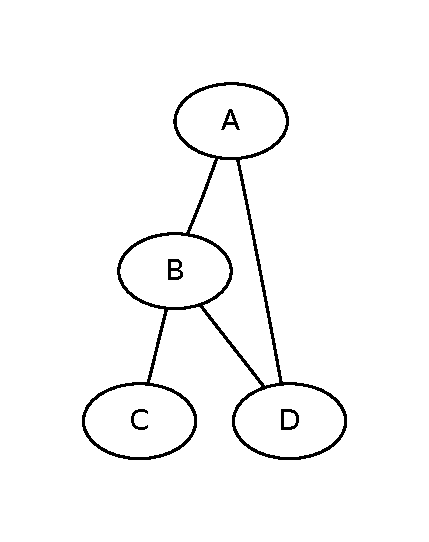
\includegraphics[width=.3\textwidth]{graphs/graph0.pdf}
\caption{Eksempel på graf}
\label{fig:graph0}
\end{figure}


\subsection{Knuder og kanter}
En graf består af knuder og kanter. Alle kanter forbinder to
knuder. En knude kan have nul eller flere kanter. Knuderne i grafen er
"`emnerne"', som grafen beskriver. Kanterne er deres relationer til
hinanden.


\begin{example}Metronettet\end{example}
  Et eksempel på en graf kunne være metronettet. Her kunne stationer
  repræsenteres som knuder og forbindelser imellem dem som kanter.

\begin{figure}[h]
\centering
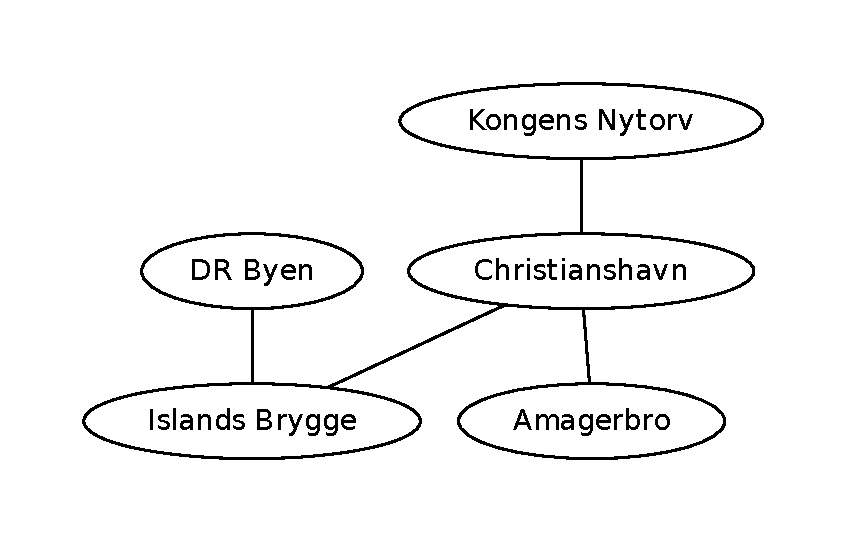
\includegraphics[width=.75\textwidth]{graphs/metro0.pdf}
\caption{Graf over et udsnit af metronettet}
\label{fig:metro0}
\end{figure}

\Fref{fig:metro0} viser en graf over metronettet med 5 knuder og 4
kanter. Knuderne er stationer og kanterne forbindelser. Grafen bruges
her til at vise hvilke stationer der er forbundet til hinanden.

Grafen kaldes retningsløs eller \textit{undirected} fordi kanterne
ikke angiver en retning. En forbindelse virker begge veje. Hvis man
kan tage toget fra Nørreport til Kongens Nytorv er det også muligt at
gå den anden vej. I en graf hvor kanterne angiver en retning (en
\textit{directed} graf) er det kun muligt at "`følge"' kanten i den
angivne retning. Forbindelsen virker kun den ene vej. Dens er
\textit{ensrettet}.

\subsection{Orienterede grafer}
En orienteret (\textit{directed}) graf er en graf hvori alle kanter
har en tilknyttet retning. Kanten kan nu kun følges i den angivne
retning. Det er dog muligt at tillade "`bevægelse"' mellem to knuder i
begge retninger, ved at tilføje to kanter: en i hver retning.

\begin{example}Metronettet udbygges med ensretning\end{example} Sæt
nu, at man vælger at bygge en ensrettet forbindelse mellem DR Byen og
Kongens Nytorv. Det er nu muligt at tage toget fra DR Byen til Kongens
Nytorv, men ikke den modsatte vej. Grafen over metronettet må dermed
laves med en orienteret graf, hvor alle kanter angiver en gyldig
retning. Ved de forbindelser, der tillader bevægelse i begge retninger
bruger vi to kanter. \Fref{fig:metro1} viser grafen fra
\fref{fig:metro0} udvidet med orientering og den nye kant.
\begin{figure}[h]
\centering
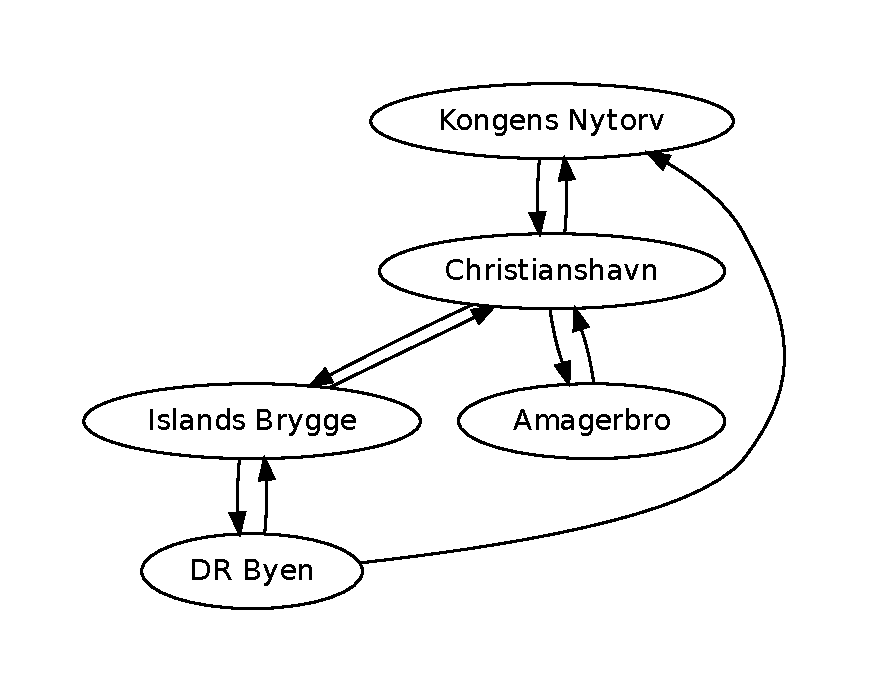
\includegraphics[width=.75\textwidth]{graphs/metro1.pdf}
\caption{Orienteret graf over metronet}
\label{fig:metro1}
\end{figure}


\subsection{Søgning i grafer}
\subsubsection{Dybde først}
\subsubsection{Bredde først}
\subsection{Korteste vej}


\section{Eksempler på grafer (Hvad kan det bruges til?!)}
\subsection{Vennenetværk (ikke-orienteret graf)}
\subsection{Telefonnumre (orienteret graf)}
\subsection{Repræsentation af en sudoku som en graf}


\section{Implementation af en graf i Python}
Nu hvor det ligger fast hvad en graf er og hvad den kan bruges det
ville det være rart med en implementation, som vi kan bruge i
Python-programmer.

I denne sektion vil vi igennem analyse (hvad skal det kunne?)
designovervejelser (hvordan skal den kunne det?) og implementation
(hvordan koder man det?) få opbygget et Python grafmodul.

\subsection{Analyse}
\label{sec:analyse}
I dette afsnit diskuteres funktionaliteten af en graf. Hvad skal den
kunne?

Kogt helt ned, skal et grafmodul besidde funktionalitet:
\begin{enumerate}
\item Oprettelse af en tom graf
\item Indsættelse af knuder i en graf
\item Sletning af knuder i en graf
\item Tilføjelse af kant mellem to knuder i en graf
\item Sletning af kant mellem to knuder i en graf
\end{enumerate}

Med disse funktioner kan vi opbygge og nedrive grafer. Men før de er
anvendelige er det nødvendigt også at kunne undersøge grafer. Følgende
funktionalitet omhandler netop dette:
\begin{enumerate}
\item Findes knude $k$ i grafen?
\item Er knude $k_1$ og knude $k_2$ forbundet af en kant?
\item Hvor mange knuder indeholder grafen?
\item Hvor mange kanter indeholder grafen?
\end{enumerate}


\subsection{Designovervejelser}
I analysen \fref{sec:analyse} gennemgik jeg funktionaliteten af en
graf. Nu vil jeg diskutere hvordan denne funktionalitet kan
implementeres i Python.

Eftersom mine funktionaliteter beskæftiger sig med en specifik instans
af en graf, vælger jeg at lave en klasse \ct{Graf}, der
repræsentere en graf med de beskrevne muligheder. Hver funktionalitet
implementeres som en metode, der arbejder på grafen.

Inden jeg kan gå i gang med at beskrive, hvordan en graf kan ændres,
skal jeg først vælge en repræsentation af en graf. Hvordan kan skal
grafobjektet holde styr på knuder og kanter?

Der er følgende traditionelle måder at gøre dette på:
\begin{enumerate}
\item Hver knude indeholder en liste af andre knuder, som den er
  forbundet til.
\item Hver kant består af et par knuder, som denne forbinder.
\item En matrix af $($knuder $\times$ knuder$)$ angiver om et given
  par er forbundet\footnote{tænk på matricen som en liste af
    lister, der hver har et element for hver knude.}.
\end{enumerate}

Den første løsning kan implementeres med en \ct{Knude}-klasse, som
beskriver en knude. Det eneste knuden skal indeholde er sin egen
værdi, samt en liste over andre knuder, som den er forbundet til. At
undersøge om to knuder er forbundet kan gøres ved at løbe deres lister
igennem og se om de har hinanden som element. Køretiden for
operationen afhænger af hvor mange elementer de to knuder er forbundet
til.

Den anden løsning kan implementeres med en \ct{Kant}-klasse der
indeholder et par af knuder (de to kunder, som kanten
forbinder). \ct{Graf}-klassen skal nu indeholde en liste af knuder
sammen med en liste af kanter. At undersøge om to knuder er forbundet
af en kant kan gøres ved at løbe listen af kanter igennem og for hver
kant undersøge om de to knuder passer med parret. Køretiden er
afhænger nu af det samlede antal kanter i grafen.

Den tredje løsning kan også implementeres med lister, selvom den er
tænkt til matricer. Her behøves hverken en \ct{Kant}- eller
\ct{Knude}-klasse. \ct{Graf}-klassen indeholder en liste af knuder,
der hver har en liste af knuder. Hvis der findes en kant fra knude
nummer $1$ til knude nummer $2$ vil det andet element i den første
liste være \ct{sand} (f.eks.: \ct{kanter[1][2] == True}). Hvis kanten
ikke findes vil værdien være \ct{falsk} (altså: \ct{kanter[1][2] ==
  False}). Køretiden afhænger (grundet valget af lister) af antaller
af knuder og bliver dermed $O(k)$.\ \footnote{med matricer kan
  køretiden reduceres til $O(1)$.}\\

Jeg vælger at implementere model nummer et på grund af dens
simplicitet. I det følgende beskriver jeg hvordan jeg implementere
hver enkelte funktionalitet.

\subsubsection{Implementation af metoder}
\paragraph{Opret tom graf}
Den tomme graf er et \ct{Graph}-objekt uden nogen tilhørende
knuder. Listen af knuder er sat til den tomme liste. En tom graf kan
oprettes ved at instansiere klassen \ct{Graph}. Dennes \ct{\_\_init\_\_}
metode sætter listen af knuder til den tomme liste:
{\small
\begin{verbatim}
class Graph:
  ...
  def __init__(self):
    self.nodes = []
\end{verbatim}}

\paragraph{Indsættelse af knude}
En knude kan indsættes med \ct{Graph}-metoden
\ct{add\_node(node)}. Metoden virker ved at tilføje den nye knude til
grafens liste over knuder:
{\small
\begin{verbatim}
class Graph:
  ...
  def add_node(self, node):
    self.nodes.append(node)
\end{verbatim}}

\paragraph{Sletning af knude}
En knude kan fjernes fra en graf med \ct{Graph}-metoden
\ct{del\_node}. Metoden virker ved at fjerne knuden fra grafens list af
knuder:
{\small
\begin{verbatim}
class Graph:
  ...
  def del_node(self, node):
    self.nodes.remove(node)
\end{verbatim}}

\paragraph{Tilføjelse af kant}
En kant fra knude $a$ til knude $b$ kan tilføjes, ved at tilføje knude
$b$ til listen over kanter i knude $a$.

{\small
\begin{verbatim}
class Graph:
  ...
  def add_edge(self, node_a, node_b):
    node_a.add_edge(node_b)
\end{verbatim}}

I \ct{Node}-klassen tilføjer \ct{add\_edge} metoden knuden til dens
liste over kanter:
{\small
\begin{verbatim}
class Node:
  ...
  def add_edge(self, node):
    self.edges.append(node)
\end{verbatim}}

\paragraph{Sletning af kant}
En kan fra knude $a$ til knude $b$ kan slettes, ved at fjerne knude
$b$ fra listen over kanter i knude $a$.

{\small
\begin{verbatim}
class Graph:
  ...
  def del_edge(self, node_a, node_b):
    node_a.del_edge(node_b)
\end{verbatim}}

I \ct{Node}-klassen fjernes knuden fra listen over kanter:
{\small
\begin{verbatim}
class Node:
  ...
  def del_edge(node):
    self.edges.remove(node)
\end{verbatim}}


\paragraph{Findes knude $k$ i grafen?}
Hvis knude $k$ ligger i grafen, ligger den i listen over knuder:

{\small
\begin{verbatim}
class Graph:
  ...
  def has_node(self, node):
    return (node in self.nodes)
\end{verbatim}}

\paragraph{Findes en kant fra knude $k_1$ til knude $k_2$?}
Hvis en kan findes fra knude $k_1$ til knude $k_2$ må knude $k_2$
ligge i listen over $k_1$'s kanter:
{\small
\begin{verbatim}
class Graph:
  ...
  def has_edge(node_a, node_b):
    return node_a.has_edge(node_b)
\end{verbatim}}

I \ct{Node}-klassen testes om \ct{node\_b} ligger i listen over kanter:
{\small
\begin{verbatim}
class Node:
  ...
  def has_edge(self, node):
    return (node in self.edges)
\end{verbatim}}

\paragraph{Hvor mange knuder indeholder grafen?}
Antallet af knuder i grafen er det samme som længden af listen over
knuder:
{\small
\begin{verbatim}
class Graph:
  ...
  def count_nodes(self):
    return len(self.nodes)
\end{verbatim}}

\paragraph{Hvor mange kanter indeholder grafen?}
Antallet af kanter i grafen er lig med antallet af fra de enkelte
knuder:
{\small
\begin{verbatim}
class Graph:
  ...
  def count_edges(self):
    count = 0
    for node in self.nodes:
      count += node.count_edges()
    return count
\end{verbatim}}

I \ct{Node}-klassen tælles antallet af kanter ved at tælle antallet af
elementer i listen over kanter:
{\small
\begin{verbatim}
class Node:
  ...
  def count_edges(self):
    return len(self.edges)
\end{verbatim}}


\subsubsection{Fejlhåndtering}
Flere af ovenstående punkter kan give en fejl. Man kan forsøge at
fjerne en knude der ikke findes, eller tilføje en kant der findes i
forvejen. I dette afsnit vil jeg belyse de metoder der kan fejle, og
udvide dem med fejlhåndtering.

\paragraph{Definition af fejl:}
Til at starte med definerer jeg fire fejltyper (\ct{exceptions}), som
grafen kan \textit{kaste} i tilfælde af fejl:
{\small
\begin{verbatim}
class NodeAlreadyExistsError(Exception):
    """ Knuden findes allerede """
    pass

class NoSuchNodeError(Exception):
    """ Knuden findes ikke """
    pass

class EdgeAlreadyExistsException(Exception):
    """ Kanten findes allerede """
    pass

class NoSuchEdgeError(Exception):
    """ Kanten findes ikke """
    pass
\end{verbatim}}

\paragraph{Implementation af fejlhåndtering:}
Jeg ændrer de problematiske metoder, så de nu kaster en af
ovenstående fejl, når en ulovlig handling forsøges.\\

Argumentet til \ct{add\_node} skal være en knude, som ikke ligger i
grafen:
{\small
\begin{verbatim}
def add_node(node):
  # Fejlhåndtering
  if node in self.nodes:
    raise NodeAlreadyExistsError(node)
  # Tilføj knuden
  self.nodes.append(node)
\end{verbatim}}

Argumentet til \ct{del\_node} skal være en knude, som findes i grafen:
{\small
\begin{verbatim}
def def_node(node):
  # Fejlhåndtering
  if not node in self.nodes:
    raise NoSuchNodeError(node)
  # Slet knude
  self.nodes.remove(node)
\end{verbatim}}

\paragraph{Smartere fejlhåndtering:}
Jeg ser, at fejlhåndteringen tager følgende form:
\begin{enumerate}
\item Undersøg om en knude eller kant findes eller ej
\item Kast fejl hvis det ikke passer med forventningen
\end{enumerate}

Ved at definere en generel metode for dette, kan jeg reducere antallet
af linjer brugt på fejlhåndtering betydeligt. Jeg definerer en
funktion for knude og en for kanter. Jeg vælger at kalde dem
\ct{ensure\_nodes} og \ct{ensure\_edges}:

\begin{samepage}
{\small
\begin{verbatim}
class Graph:
  ...

  def ensure_nodes(self, nodes, must_exist):
      """ Kast en fejl hvis en af knuderne findes/ikke findes """
      for node in nodes:
          exists = self.has_node(node)
          if must_exist and not exists:
              raise NoSuchNodeError(node)
          if not must_exist and exists:
              raise NodeAlreadyExistsError(node)

  def ensure_edges(self, edges, must_exist):
      """ Kast en fejl hvis en af kanterne findes/ikke findes """
      for node_a, node_b in edges:
          exists = self.has_edge(node_a, node_b)
          if must_exist and not exists:
              raise NoSuchEdgeError((node_a, node_b))
          if not must_exist and exists:
              raise EdgeAlreadyExistsError((node_a, node_b))
\end{verbatim}}
\end{samepage}


Jeg kan nu skrive fejlhåndteringen for \ct{add\_node} og \ct{del\_node}
således:

{\small
\begin{verbatim}
def add_node(node):
  # Fejlhåndtering
  self.ensure_nodes( [node], True )
  # Tilføj knuden
  self.nodes.append(node)

def def_node(node):
  # Fejlhåndtering
  self.ensure_nodes( [node], False )
  # Slet knude
  self.nodes.remove(node)
\end{verbatim}}

Bemærk, at der kun bruges en enkelt linje til fejlhåndtering i den nye
kode. Jeg fortsætter med at tilføje fejlhåndtering til de andre
kritiske metoder: \\

Argumenterne til \ct{add\_edge} skal være to knuder, der findes i
grafen (der må gerne findes en kant i forvejen):
{\small
\begin{verbatim}
class Graph:
  ...
  def add_edge(self, node_a, node_b):
    # Fejlhåndtering
    self.ensure_nodes(  [node_a, node_b]  , True  )
    # Tilføj kant
    node_a.add_edge(node_b)
\end{verbatim}}

Argumenterne til \ct{del\_edge} skal være to knuder, der deler en
kant:
{\small
\begin{verbatim}
class Graph:
  ...
  def del_edge(self, node_a, node_b):
    # Fejlhåndtering
    self.ensure_edges( [(node_a, node_b)], True )
    # Slet kant
    node_a.del_edge(node_b)
\end{verbatim}}

\subsection{Endelig Implementation}
\begin{alltt}
\input{code/graph.py}
\end{alltt}

\subsection{Test og afprøvning}

\end{document}

